% ---- pg-083 （书页 71） ----

一般的,
\[
\left|\begin{matrix} a_{11} & a_{12} \\ a_{21} & a_{22} \end{matrix}\right| = a_{11}a_{22}(-1)^2 + a_{12}a_{21}(-1)^3 = a_{11}a_{22} - a_{12}a_{21}
\]
\[
\left|\begin{matrix} 3 & 1 & 6 \\ 7 & 4 & 5 \\ 2 & -7 & 1 \end{matrix}\right|
= 3\left|\begin{matrix} 4 & 5 \\ -7 & 1 \end{matrix}\right|(-1)^2
+ 1\left|\begin{matrix} 7 & 5 \\ 2 & 1 \end{matrix}\right|(-1)^3
+ 6\left|\begin{matrix} 7 & 4 \\ 2 & -7 \end{matrix}\right|(-1)^4
\]
\[
= 3\times39 - 1\times(-3) + 6\times(-57) = -222
\]
\[
\left|\begin{matrix} 1 & 0 & 0 \\ 0 & 1 & 0 \\ 0 & 0 & 1 \end{matrix}\right|
= 1\left|\begin{matrix} 1 & 0 \\ 0 & 1 \end{matrix}\right|(-1)^2
+ 0\left|\begin{matrix} 0 & 0 \\ 0 & 1 \end{matrix}\right|(-1)^3
+ 0\left|\begin{matrix} 0 & 1 \\ 0 & 0 \end{matrix}\right|(-1)^4
\]
\[
= 1\times1 = 1
\]

如果 $\bm{I}$ 是 $k\times k$ 单位矩阵,则 $|\bm{I}| = 1$.
\[
\left|\begin{matrix} a_{11} & a_{12} & a_{13} \\ a_{21} & a_{22} & a_{23} \\ a_{31} & a_{32} & a_{33} \end{matrix}\right|
\]
\[
= a_{11}\left|\begin{matrix} a_{22} & a_{23} \\ a_{32} & a_{33} \end{matrix}\right|(-1)^2
+ a_{12}\left|\begin{matrix} a_{21} & a_{23} \\ a_{31} & a_{33} \end{matrix}\right|(-1)^3
+ a_{13}\left|\begin{matrix} a_{21} & a_{22} \\ a_{31} & a_{32} \end{matrix}\right|(-1)^4
\]
\[
= a_{11}a_{22}a_{33} + a_{12}a_{23}a_{31} + a_{21}a_{32}a_{13} - a_{31}a_{22}a_{13} - a_{21}a_{12}a_{33} - a_{32}a_{23}a_{11}
\]

任一 $3\times3$ 矩阵的行列式可按下面图形计算,即沿实线方向的元素乘积相加,再减去沿虚线方向的元素乘积.这种方法对更高维数的矩阵不成立.不过,一般可利用定义 2A.24 来计算更高维数的情况.

下面我们将要陈述的结论描述了行列式的一些性质.但是,必须先引入与逆矩阵有关的概念.

\begin{mvfigure}
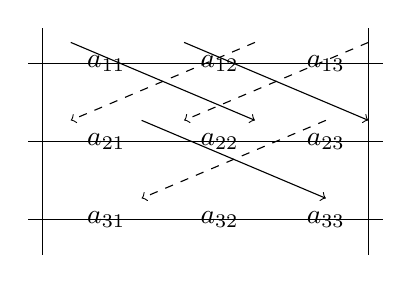
\begin{tikzpicture}[scale=0.9]
% three horizontal lines
\draw (0,2.6) -- (5.0,2.6);
\draw (0,1.5) -- (5.0,1.5);
\draw (0,0.4) -- (5.0,0.4);
% vertical-ish separator lines
\draw (0.2,3.1) -- (0.2,-0.1);
\draw (4.8,3.1) -- (4.8,-0.1);
% nodes
\node at (1.1,2.6) {$a_{11}$};
\node at (2.7,2.6) {$a_{12}$};
\node at (4.2,2.6) {$a_{13}$};
\node at (1.1,1.5) {$a_{21}$};
\node at (2.7,1.5) {$a_{22}$};
\node at (4.2,1.5) {$a_{23}$};
\node at (1.1,0.4) {$a_{31}$};
\node at (2.7,0.4) {$a_{32}$};
\node at (4.2,0.4) {$a_{33}$};
% solid arrows (down-right)
\draw[->] (0.6,2.9) -- (3.2,1.8);
\draw[->] (2.2,2.9) -- (4.8,1.8);
\draw[->] (1.6,1.8) -- (4.2,0.7);
% dashed arrows (down-left)
\draw[dashed,->] (4.8,2.9) -- (2.2,1.8);
\draw[dashed,->] (3.2,2.9) -- (0.6,1.8);
\draw[dashed,->] (4.2,1.8) -- (1.6,0.7);
\end{tikzpicture}
\end{mvfigure}

\mvthm{定义 2A.25}{如果把一个矩阵的行看成向量(即行向量),矩阵的行秩就是线性无关的行的最大数目.如果把矩阵的列看成向量,一个矩阵的列秩是它的列集合的秩.}

例如,设矩阵
\[
\bm{A} = \begin{bmatrix} 1 & 1 & 1 \\ 2 & 5 & -1 \\ 0 & 1 & -1 \end{bmatrix}
\]

把 $\bm{A}$ 的行写成向量形式,定义 2A.6 后的例子已证明它们是线性相关的.注意 $\bm{A}$ 的列秩也是 2,因为
